\documentclass[12pt,a4paper]{article}
  \usepackage[toc,page]{appendix}
  \usepackage{longtable}
  \usepackage{listings} 
  \usepackage{verbatim}
  \usepackage{graphicx}
  \usepackage{tabularx}
  \usepackage{subfig}
  \usepackage{float}
  \usepackage{pdfpages}
  \usepackage{csvsimple}
  \usepackage[a4paper,bindingoffset=0.2in,left=0.6in,right=0.6in,top=1in,bottom=1in,footskip=.25in]{geometry}
  \begin{document}
    \begin{titlepage}
      \centering
      {\scshape\LARGE Goldsmiths, University of London \par}
      \vspace{1cm}
      {\scshape\Large Software project final report\par}
      \vspace{1.5cm}
      {\huge\bfseries iLost\par}
      \vspace{2cm}
      {\Large\itshape 
        Ahmed, Muhammad\\
        Chowdhury, Thairan\\
        Davies Minta, Dylan\\     
        Fakrul, Mahmudul\\    
        Farkhani, Hussein\\ 
        Jheng-Hao, Lin\\
        Pecorella, Mariano\\ \par}
      \vfill
      supervised by\par
      \textsc{Tim Blackwell} 
      \vfill
      % Bottom of the page
      {\large \today \par}
    \end{titlepage}

    \tableofcontents
    \newpage

    \section{Introduction}
    \section{Development Record}
    \newpage
    \section{Formative Evaluation}
      % total 1650 words
      \subsection{iOS App Evaluation} 
          % total 1000 words
        \subsubsection{Objectives and Questions}
          % 100 words
          \paragraph{}
            We wrote quantitative tasks to test the usability of our mobile application\cite{WritingTasks}. The purpose of the tests was to test if the participants can actually finish the task with the application, and we could learn from the process to observe how users used our application and improve it if any issue or confusion was raised. 

            \begin{figure}[H]
              \centering
              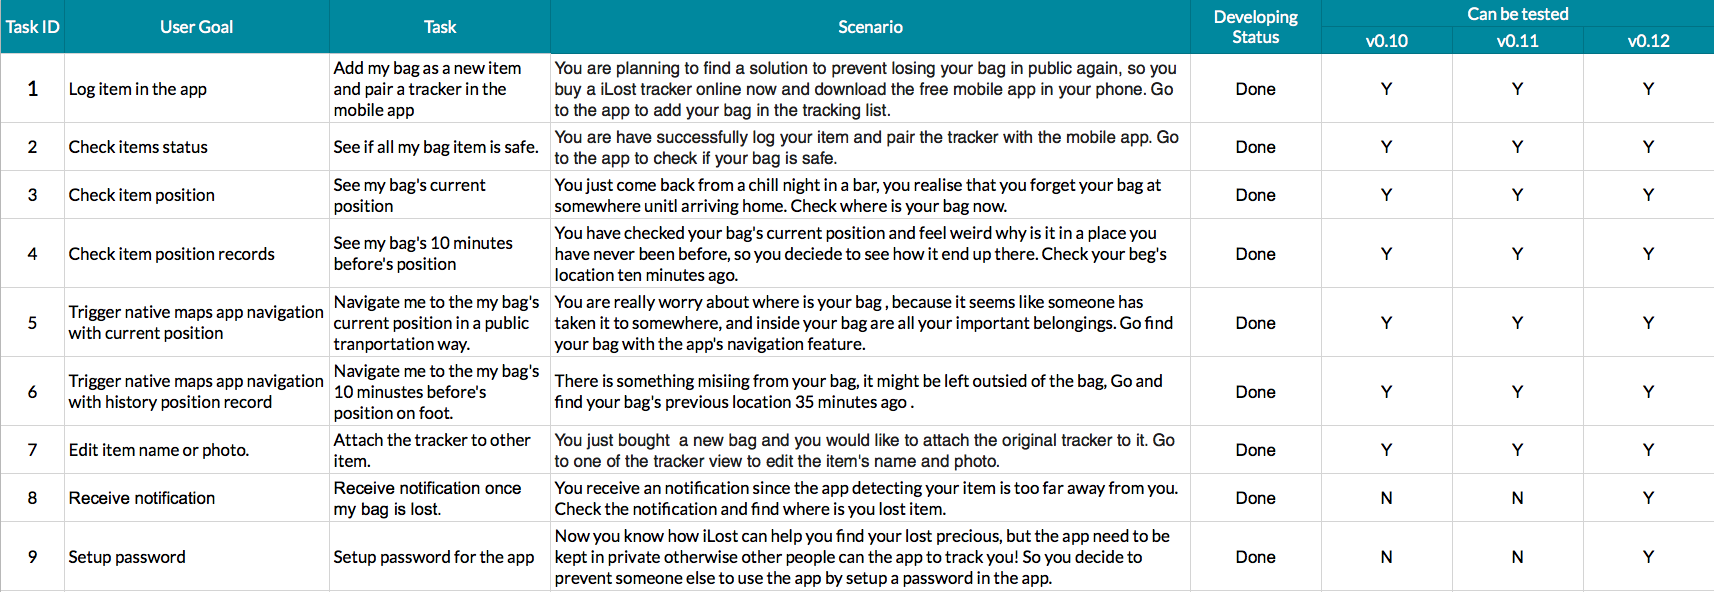
\includegraphics[width=1\textwidth]{../assets/usability-test-task-list.png}
              \caption{Usability test task list}
              \label{fig:Usability test task list}
            \end{figure}

            \begin{table}[H]
              \centering
                \begin{tabularx}{\textwidth}{l X}
                  \hline
                  Column & Description  \\ \hline
                  Task ID & Identify number of the task  \\ 
                  User Goal & What is the objective we need users to perform.  \\ 
                  Task & The process in terms of completing the goal  \\ 
                  Scenario & A setup scenario for engaging testers to use the application in a real-life case.   \\ 
                  Developing Status & Current latest developing status of the functionality of this task, it should be {\bf To do}, {\bf In Progress} and {\bf Done}.\\ 
                  Can be tested &  Whether the functionality of the application is ready to be tested in each version.\\ 
                  \hline
                \end{tabularx}
                \caption[Table caption text]{Usability test task list columns}
                \label{table:Usability test task list columns}
            \end{table}

            Figure \ref{fig:Usability test task list} demonstrates our tasks and goals. The table \ref{table:Usability test task list columns} shows what the columns stand for.

        \subsubsection{Participants, Location and Setup}
          % 100 words
          \paragraph{} According to Jakob Nielsen, testing 5 users in a usability study could find almost as many usability problems as testing more participants\cite{HowManyTestUsers}. So application was tested with 5 participants for each version. The study was taken place in the library of the Goldsmiths, University of London, and the participants were the students who used to bring a bag to the campus daily. Totally we have conducted three versions of the application.
          
        \subsubsection{Methodology and Measures}
          % 100 words
          \paragraph{} Firstly, we explained what was our project about and asked participants to sign up the consent form which can be found in appendices \ref{appendix:consent-form}. During the test, the participants were provided an iPhone with the application built-in to test. An observer would guide them through the tasks and the scenarios, then took notes of how the participants reacted to the application. For each task, the observer would record it was successfully completed or failed. The records would help us to build the success rates diagram which helped us to understand which usability needed to be improved\cite{SuccessRates}. 

        
        \subsubsection{Evaluations}
          
          \begin{figure}[H]
            \centering
            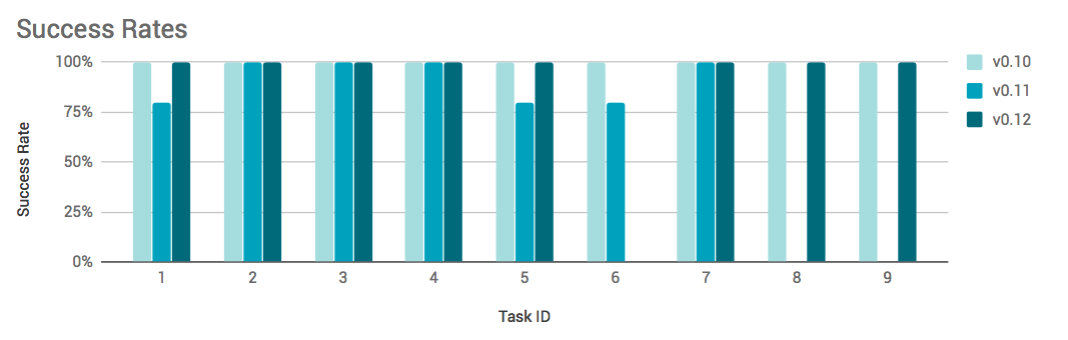
\includegraphics[width=1\textwidth]{../assets/usability-test-success-rates.png}
            \caption{iOS App Success Rates Diagram}
            \label{fig:iOS App Success Rates Diagram}
          \end{figure}

          \paragraph{v0.10} The tested subject was the application prototype built in {\bf Adobe XD}, which was one of the best design tools to test the prototype. Thanks to the well-designed user interfaces, the goals were easy to achieved and all the tasks were all succeeded. The result could only prove that the user interfaces guided the users to the right view, but it could not actually reflect on the usability of the real application. After all, Adobe XD could only let users walk through each view by clicking, while an actual iOS application should support swipe or other gestures. It was more like a paper prototype usability test.
          
          \paragraph{v0.11} We benefited most from this test since this test was the native mobile application we where the participants can actually use it like other application. This version was built in React Native and tested in Expo which a tool and service which we used to build the mobile native application with React Native. During this test, we received several comments towards the {\bf add item view}. For example, the camera icon in that view was originally used as a button. But some of the users could not really regard it as a button but a decoration since it was colourful. Also, the placeholder of the item name field was {\bf Item Name} instead of a prompt message which confused some of the participants as well. So after this test, we resolved the issues and the difference shows in figure \ref{fig:usability-test-ios-v010-improvements}. The task 8 and 9 were not developed completely at the moment so there was not any record.

          \begin{figure}[H]
            \centering
            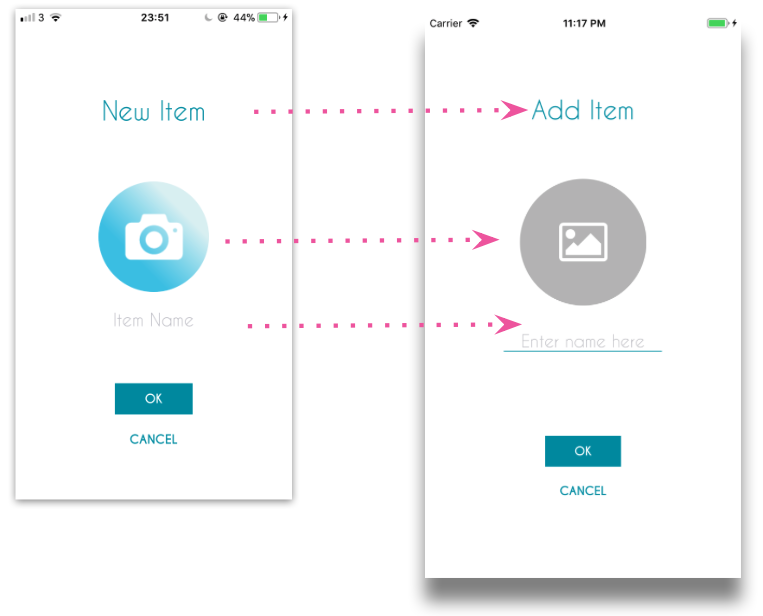
\includegraphics[width=0.7\textwidth]{../assets/usability-test-ios-v010-improvements.png}
            \caption{Improvement of the add item view}
            \label{fig:usability-test-ios-v010-improvements}
          \end{figure}

          \paragraph{v0.12} After the previous test, we not only improved some of the user interfaces but also removed some of the features. It is worth notice that there is no record of task 6, which is {\bf navigating to previous locations of the item's location history}. The reason we removed this task was that this goal was not really helpful. The participants commented that it was not beneficial to navigate to the previous locations, they cared about the current location of the item more. So thanks to the feedback, we removed the task 6 and eliminated the functionality of navigating through history locations which made the application more simple. 
        
        \subsection{Tracker Evaluation}
            total 700 words
          \subsubsection{Objectives and Questions}
            100 words
          \subsubsection{Location, Setup and Participants}
            100 words
          \subsubsection{Methodology and Measures}
            100 words
          \subsubsection{Tracker v0.10 Evaluation}
            150 max words
          \subsubsection{Tracker v0.11 Evaluation}
            150 max words
        \subsection{Conclusion}
          % 200 max words
          Even though the tasks could be completed, but in terms of the user experience, we still had space to improved. 
      \newpage
    \section{Design and Implementation}
    \section{Quality Assurance}
    \section{Summative Evaluation}
    
    \begin{thebibliography}{20}
      % \addcontentsline{toc}{chapter}{Bibliography}
      \bibitem{HowManyTestUsers} "How Many Test Users in a Usability Study?", Nielsen Norman Group, 2012. [Online]. Available: https://www.nngroup.com/articles/how-many-test-users/. [Accessed: 01- Mar- 2018].
      \bibitem{WritingTasks} "Writing Tasks for Quantitative and Qualitative Usability Studies", Nielsen Norman Group, 2018. [Online]. Available: https://www.nngroup.com/articles/test-tasks-quant-qualitative/. [Accessed: 14- Mar- 2018].
      \bibitem{SuccessRates} "Success Rate: The Simplest Usability Metric", Nielsen Norman Group, 2001. [Online]. Available: https://www.nngroup.com/articles/success-rate-the-simplest-usability-metric/. [Accessed: 14- Mar- 2018].
    \end{thebibliography}
    
    \begin{appendices}            
      \section{Development Records}
        \subsection{Tasks Divided}
        \subsection{Progress Tracking Form}
      \section{Formative Evaluation}
        \subsection{consent Form}
          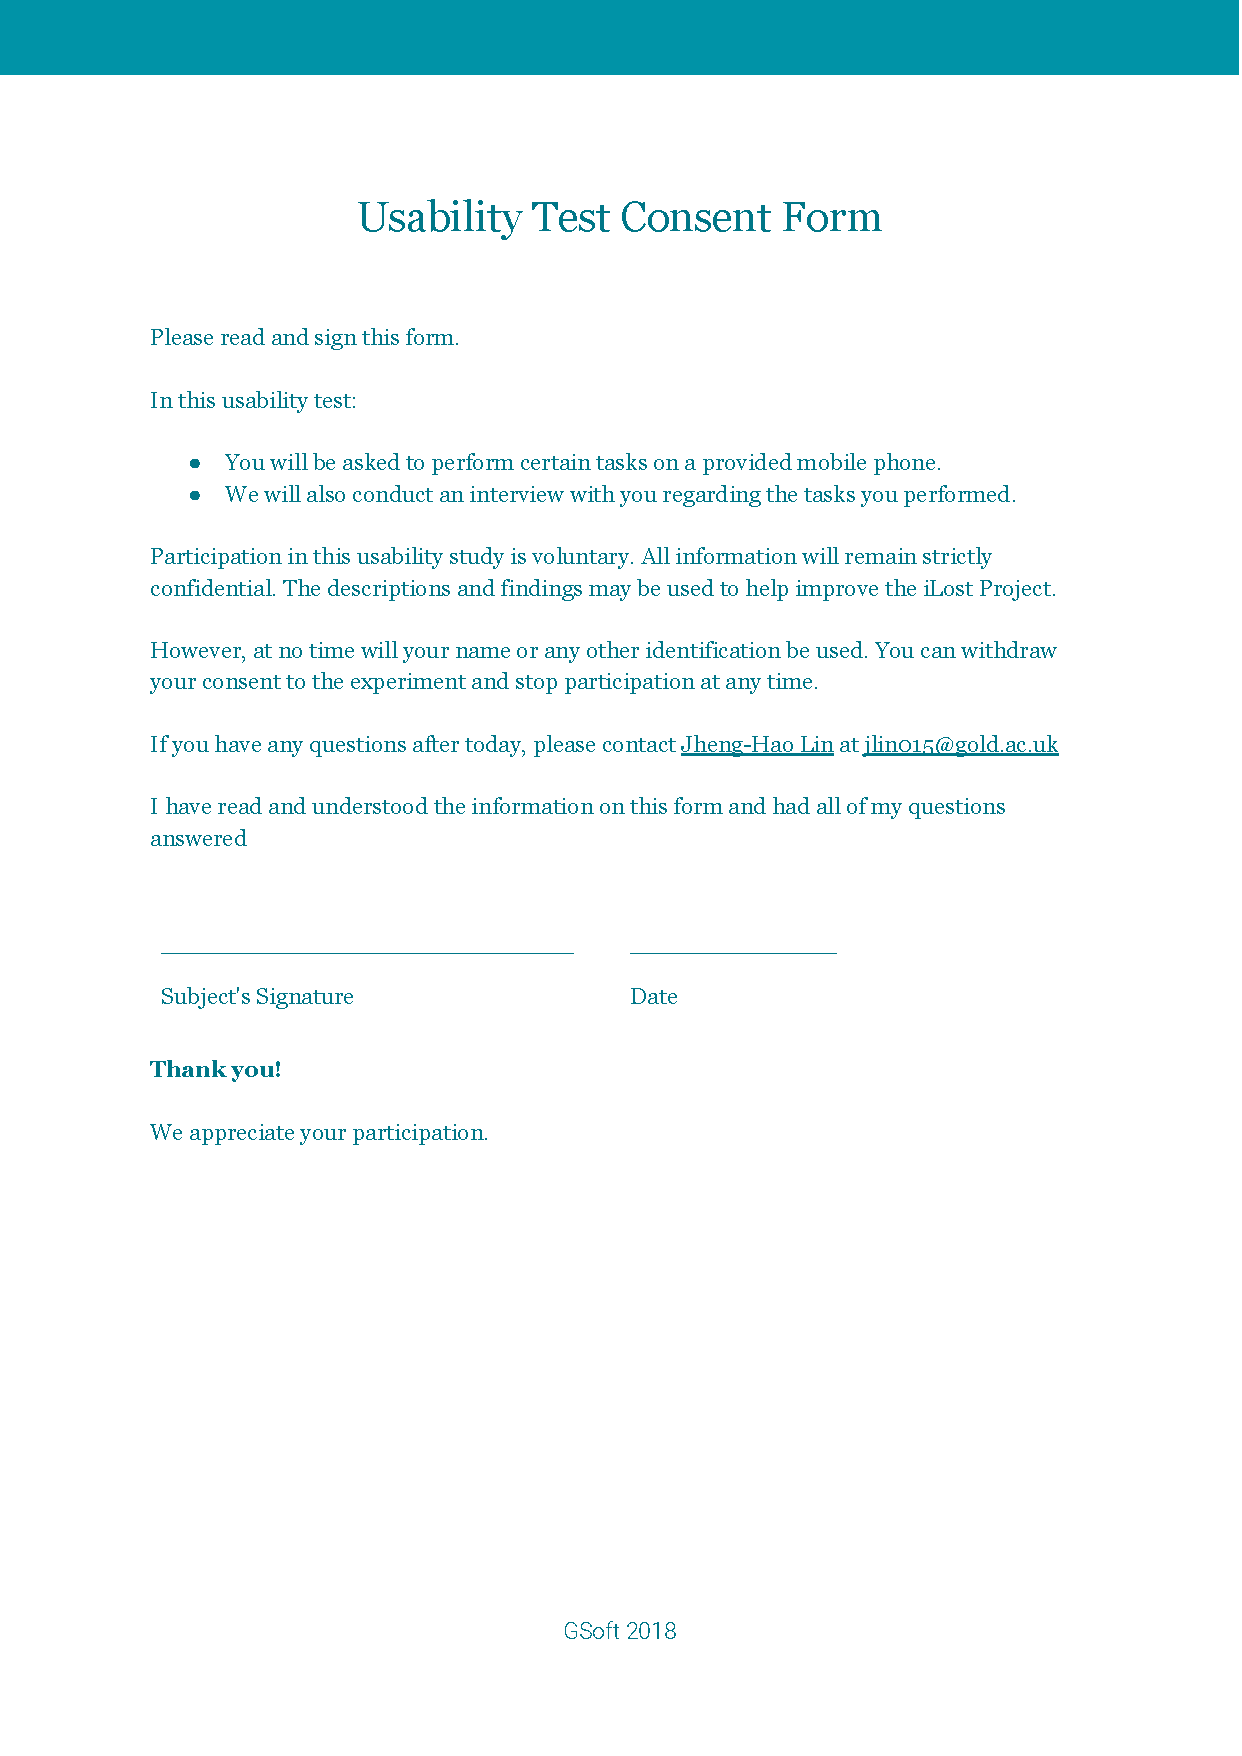
\includepdf[pages={1}]{../assets/usability-test-consent-form-example.pdf}
          \label{appendix:consent-form}
      \section{Design and Implementation}
        
      \section{Quality Assurance}

    \end{appendices}

  \end{document}


